\section{Design of Architecture} \label{sec:overview}

Figure 2 shows our proposed architecture in KVM virtualization environment. 
It contains three main components: the Serviceguard, a tailored version 
of QEMU, and the \smr system \smrsystem. 
Only the primary VM advertises its presence on the network, so all network 
inputs come to the primary VM. 
The Serviceguard is deployed on the virtual machine, and provides monitoring 
capabilities for applications running inside virtual machines in the KVM 
virtualization environment.

\begin{figure}[t]
% \vspace{.20in}
\centering
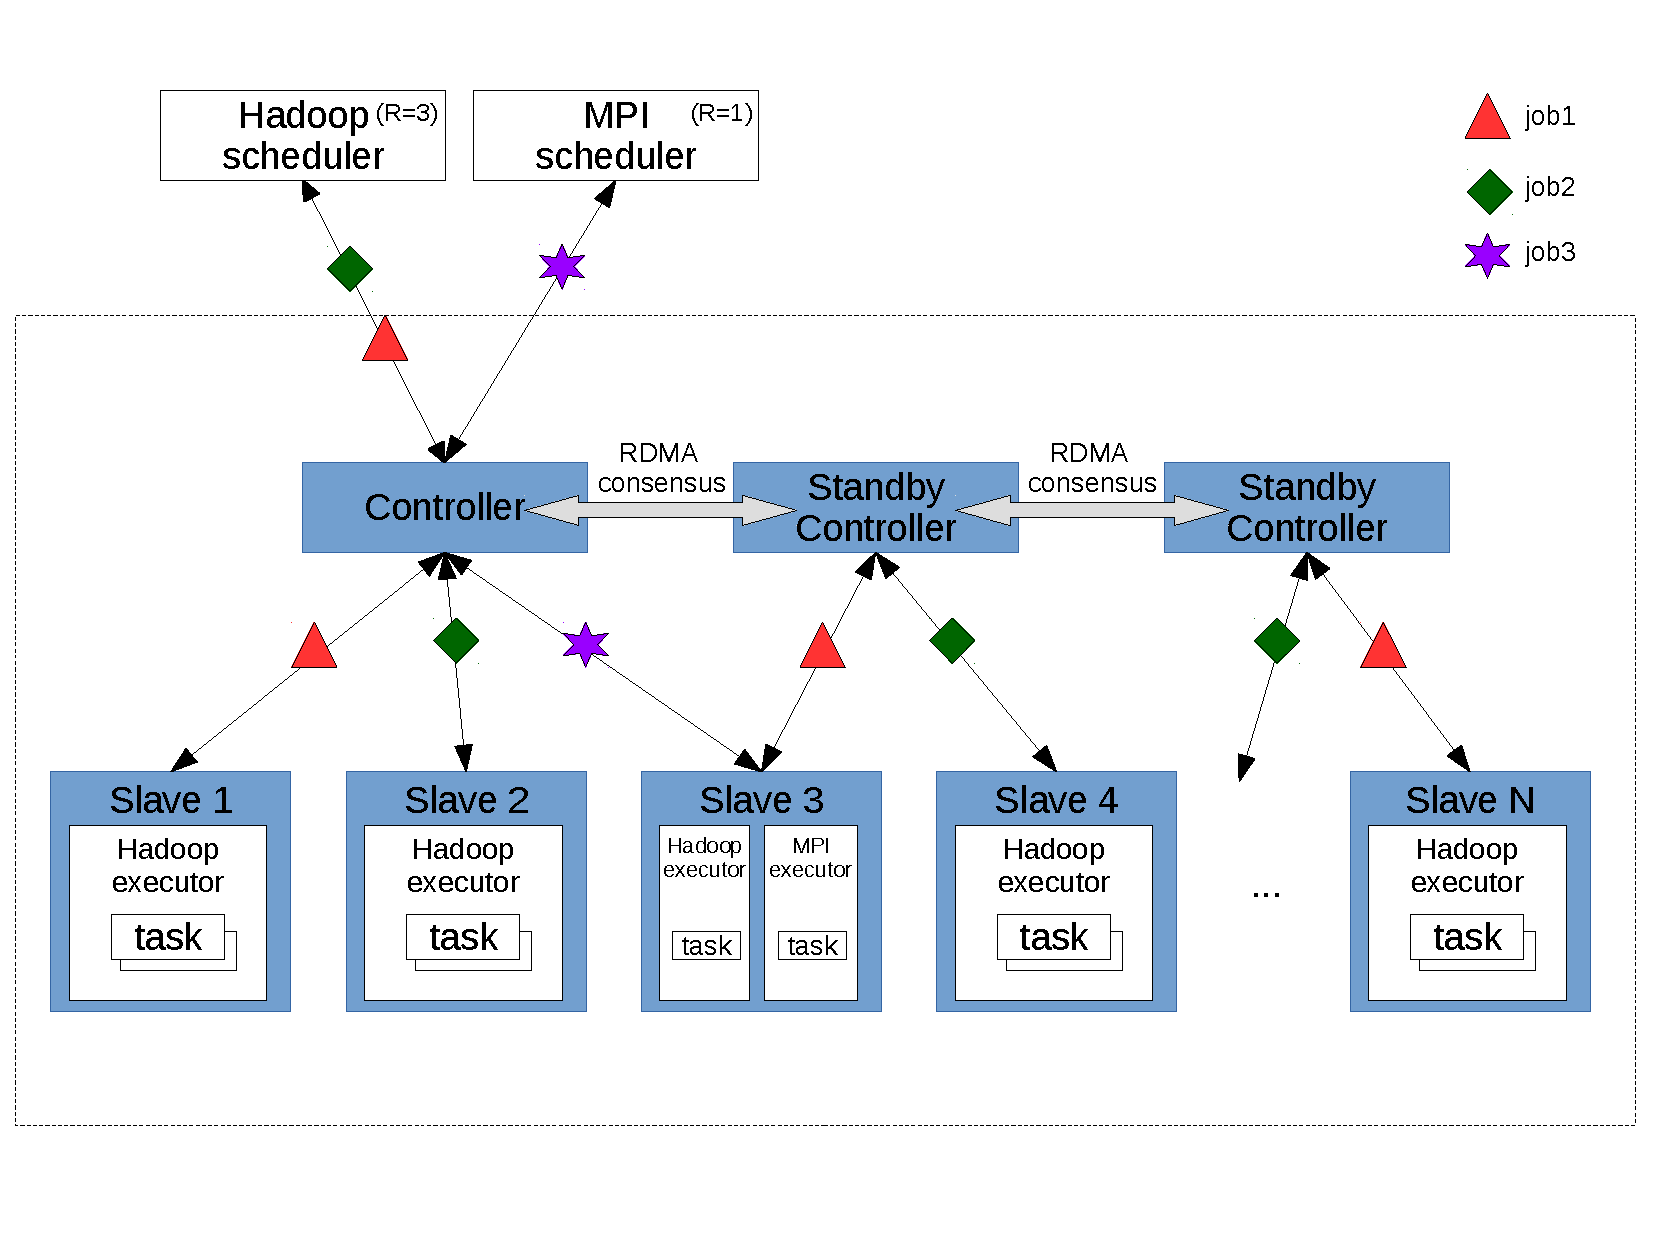
\includegraphics[width=.47\textwidth]{figures/arch}
\vspace{-.2in}
\caption{{\em Proposed architecture in KVM virtualization environment.} Key 
components are shaded (and in blue).} \label{fig:arc}
\vspace{.05in}
\end{figure}
